\section{Scheduability Analysis Modeling}
\label{sec:ScheduabilityAnalysisModeling}

	In this section we want to investigate the encapsulated EDF-scheduler (earliest deadline first scheduler) from the schedulig procedure by Kaiser \cite{K}. It is homogeneous multiprocessor systems comprising $m\in \mathbb{N}$ processors.\\


%%%%%%%%%%%%%%%%%%%%%%%%%%%%%%%%%%%%%%%%%%%%%%%%%%%%%%%%%%%%%
% Brief introduction to multiprocessor scheduling
% prework of the PROSA implementation
%%%%%%%%%%%%%%%%%%%%%%%%%%%%%%%%%%%%%%%%%%%%%%%%%%%%%%%%%%%%%

\subsection{Taxanomie of Multiprocessor Scheduling Algorithms}
\label{subsec:TaxanomieOfMultiprocessorSchedulingAlgorithms}

	Let's recap \glspl{real-time system} as given in \cite{KBK}.
	And compare it with the classification given in \cite[section 2.3]{DB2011}.
	The {\itshape process} or {\itshape task} is defined as an sequential execution of a {\itshape program}  or {\itshape job} on a processor.
	The execution ends after a \emph{finite number} of steps.
	Therefore the execution corresponds to a finite execution of machine commands and is not separable.\\
	
	\begin{lemma}
		\label{remark:problems}
		Multiprocessor scheduling can be viewed as attempting to solve two problems.
		\begin{enumerate}[label=(\roman*)]
			\item The \emph{allocation problem}, or on which processor the task should execute.
			\label{remark:allocationproblem}
			\item The \emph{priority problem}, or in what order with respect to jobs of tasks each job should be executed.
			\label{remark:priorityproblem}
		\end{enumerate}
	\end{lemma}
	
	
	\begin{definition}
		 A process is called periodic if it should be restated after a certain time called the period.
		 \begin{enumerate}[label=(\roman*)] 
		\item Otherwise a process is called aperiodic or sporadic.
		\item Furthermore, whenever as process is said to be non-preemptive the execution may not be interrupted between the beginning and ending of the process. 
			  A process is called preemptive if it may be interrupted after any instruction.
		\end{enumerate}
		\end{definition}  
	 
	The slotted priority modell is from Bollela \cite{B97} with  sporadic and periodic processes (\cite{K}).
	Due to \cite{B97} the major requirement is said to be as in the following:
	
	\begin{quote}
		`If a system itselves the execution of a real-time and non-real-time thread in alternate intervals the intervals in which real-time threads execute are scheduled to be in every $l$ time unit, then it must be ensured that the interval begin at time $t$ where $kl \leq t \leq kl+\epsilon \quad \forall \epsilon \geq 0$'.
	\end{quote}
	
	Roughly speaking there should be a covering of the time $t$ with a diameter of $\epsilon$ for each positive $\epsilon$.
	Moreover there is this requirement labeld by  $\mathcal{B}$ \cite{B97}.
	\begin{quote}
		`For $L>\epsilon$ (for a suitable $\epsilon$) for which the real-time thread schedule has asserted a real-time thread $\tau$ to be executed on the CPU, there must be a function of the method by which the minimum number of CPU cycles available to execute the instructions of $\tau$ can be determined.'
	\end{quote}
	But it is apriory not clear what this number $L$ might be and how this CPU-cycle number is determined.
	
%%%%%%%%%%%%%%%%%%%%%%%%%%%%%%%%%%%%%%%%%%%%%%%%%%%%%%%%%%%%%%	
	\paragraph*{Encapsulation of a scheduled process}
	\label{par:EncapsulationOfAScheduledProcess}
%%%%%%%%%%%%%%%%%%%%%%%%%%%%%%%%%%%%%%%%%%%%%%%%%%%%%%%%%%%%%%
	 
		The scheduler found in \cite{K} is going to be classified for the scope of implementation. 
		We follow the paper \cite{DB2011} which gives a survey of hard real-time systems.
		It is an encapsulated priority based (see Remark \ref{remark:problems}, \ref{remark:priorityproblem}), fixed job priority,   EDF (earliest-deadline-first) process with scheduling inside the representative (global) process.
	
	
	\begin{figure}[h]
		\centering
		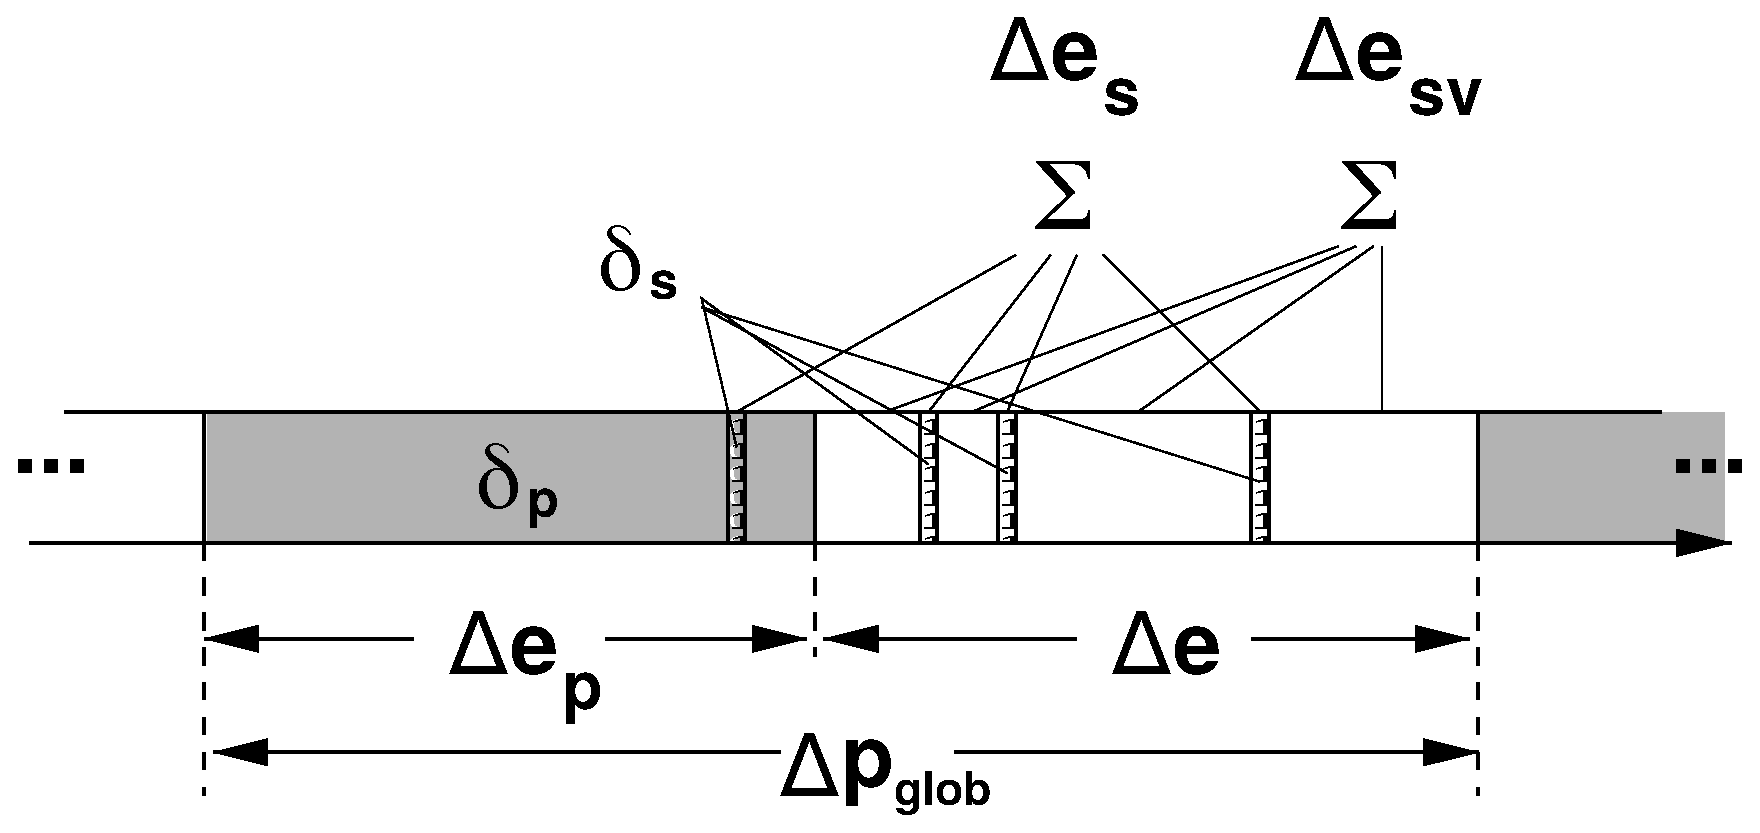
\includegraphics[width=0.7\textwidth]{timeslot_and_disruptive_process.eps}
		\caption{Timeslot partitioning of  $\Delta e_s, \Delta e_p$, $\Delta e_{sv}$ and $\Delta_e$ of the disruptive process $\delta_s$ and $\delta_p$, Source: \cite{K}}
		\label{fig:timeslots}
	\end{figure}
	
	\begin{definition}
		\begin{subequations}     
			\begin{align} 
				Let \quad & \delta_p \in \mathbb{N} \quad \text{denote a periodic disruptive process and}\\
	 	&\delta_s \in \mathbb{N} \quad \text{denote a asporadic disruptive process.}
	 		\end{align}
		\end{subequations}
	\end{definition}
	 	
	\begin{definition}
	 	\begin{subequations}
	 		\begin{align}
	 \text{Let} \quad P& := \{1, \cdots, n \} \subset \mathbb{N}^n \quad \text{be a job,}\\
	  &\text{a set of interruptible processes with fixed priority order ascading.} \\
	 	\text{Let} \quad \delta p_i &\in \mathbb{N}, \quad \text{for} \quad i = 1,..,n \quad  \text{denote the period and}  \\
	 	&\delta e_i  \in \mathbb{N} \quad \text{for} \quad  i = 1,..,n \quad  \text{denote the execution time of a proces}.  
	 		\end{align}   
	 	\end{subequations}
	\end{definition}
	
	\begin{theorem}
	 	\begin{subequations}
	 		\begin{align}
	 		\text{Let} \quad P &=\{1, 2, \cdots,n \} \text{ be job scheduled by RTS} \\
	 		\text{for} \quad \Delta P_A & \geq  \Delta p_{grob} \text{we have}\\
	        \quad P' &:= \{\delta_p, \delta_1, 1, \cdots, n \} \subset \mathbb{N}^{(n+2)} \quad \text{is scheduled by RTS}.
	  		\end{align}   
	 	\end{subequations}
	\end{theorem}
	
	Moreover, we define the slotted priority model by Bollella with Kaiser's sporadic and periodic disruptive process with a discrete time in contrast to these authors.
	This chioce is due to the real-time kernel from \cite{PROSA_schedubility_analysis} and the real-time kernel model as in \cite[chp. 5.3]{B97} and the exclusion model \cite[p.12]{B97}.
	
	\begin{definition}
		Time is $\mathbb{N}$.
	\end{definition}
	
	\begin{definition}
		The utilization of the i-th process is given by 
		\begin{equation} 
		U(i) = \frac{\delta e_i}{\delta p_i}- 
		\end{equation}
	\end{definition}
	\begin{lemma}
	$U(i)$ is well-defined.
	\end{lemma}
	\begin{proof}
	For every $i\in \mathbb{N}$, $U(i)$ is the quotient of two positive numbers.
	\end{proof}
	
	\begin{definition}
	The utilization of the process set $P$ is given by 
		\begin{equation}
		U(P)= \sum_{i=1}^n \frac{\delta e_i}{\delta p_i}.
		\end{equation}
	\end{definition}
	
	According to \cite{B97} due to establishing the exclusion model we denote  a scheduling function in the following way:
	
	\begin{definition}
	We say a multiprocessor scheduling algorithm $\sigma$ is given by 
		\begin{align} 
		\sigma: &\mathbb{N}^n \times \mathbb{N}^n \longrightarrow  \mathbb{N} \times \{1,2,\cdots, m\} \\
		&\forall i, \delta e_j \in  \mathbb{N} \quad (i ,\delta e_j)  \mapsto (t,k) \in \mathbb{N}\times \{1,2,\cdots,m\}. 
		\end{align}
	\end{definition}
	
	\begin{definition}
	Let $P_i\in \mathcal{P}$ be a process and 
	\begin{equation}
	P^j_i = ( \delta p_i, r_i) \in \mathbb{N}_o^2,  
	\end{equation}
	where $\delta p_i$ is called the period and $r_i$ the residuum. 
	\end{definition}
	Furthermore, time controlled process allocation similarly as \cite{B97} and \cite[p. 34]{K} is defined as in the following. In contrast to these authors time is discrete.
	
	\begin{definition}
	Let $\sigma_T: \mathbb{N} \times \mathbb{N} \rightarrow \mathbb{N}_0$ be a function called the time schedule or implementation plan.
	\begin{enumerate}
	\item $\forall t \in \mathbb{N}$ we have $\sigma_T(t)\in \{1,2,...,n\}$
	\item \begin{equation}
			\sigma_T(t,\delta e_j) =
			\begin{cases}
				k > 0 & \text{we say the process $P_k$ is working at time $t$.}\\
				0 & \text{the process is not working.}\\
				  &\quad  \text{Then the idele-process$i$ of the operating system is working.}
			\end{cases}       
	\end{equation}
	\end{enumerate}
	\end{definition}
	
	A depute process is given by $ N = \{1, \cdots, n\}\subset \mathbb{N}$. 
	
	Let $P \subset \{1, \cdots, n\} \subset S$.
	$S$ is executed in a periodically repeated timeslot such that $\delta p_{sv}$ is the periodlength and $\delta e_{sv}$ is the size of the time slot (see Figure \ref{fig:timeslots}).
	The remaining period time is contains the  disruptive process $\delta_p$ and $\delta_s$.
	
	We are writing
	\begin{align}
		\Delta p_{sv} &\text{ for the period length} \\
		\Delta e_s &\text{ for the execution time of the sporatic process and}\\ 
		\Delta e_p &\text{ for the execution time of a periodic task.}
	\end{align}
	
%%%%%%%%%%%%%%%%%%%%%%%%%%%%%%%%%%%%%%%%%%%%%%%%%%%%%
	\paragraph{The slotted priority model by Bollela}
	\label{par:TheSlottedPriorirtyModelByBollela}
%%%%%%%%%%%%%%%%%%%%%%%%%%%%%%%%%%%%%%%%%%%%%%%%%%%%%
	
	Within this model we are having a two-staged process hirachie. 
	The global scheduler is purely time-controlled.
	Its' period is given by $\Delta p_{glob}$ and its' execution task time slot is still to remain $\Delta e_{time}$.
	The representative process is the local scheduler. 
	It is non interruptable, periodic disruptive process.
	We have
	\begin{align}
	\Delta e_p &:= \Delta p_{glob} - \Delta e\\
	\Delta p_{p} &:= \Delta p_{glob}, 
	\end{align}
	where $\Delta p_{p}$ denotes the period of the disruptive process.
	
%%%%%%%%%%%%%%%%%%%%%%%%%%%%%%%%%%%%%%%%%%%%%%%%%%%%
	\paragraph{The sporadic disruptive process}
	\label{par:TheSporadicDisruptiveProcess}
%%%%%%%%%%%%%%%%%%%%%%%%%%%%%%%%%%%%%%%%%%%%%%%%%%%%
	
	As in \cite{K} the sporadic des
	ptive process with cumulated calculation time $\Delta e$ satisfies
	\begin{equation}
	\Delta p_{p} \leq \lvert{\Delta p_{glob}} \rvert. 
	\end{equation}
	
%%%%%%%%%%%%%%%%%%%%%%%%%%%%%%%%%%%%%%%%%%%%%%%%%%%%
	\paragraph{Model of a sporadic disruptive process}
	\label{par:ModelOfASporadicDisruptiveProcess}
	
%%%%%%%%%%%%%%%%%%%%%%%%%%%%%%%%%%%%%%%%%%%%%%%%%%%%%%%%
	
	We say we are talking of a slotted priority model if the 
	
	\begin{remark}
	Note that $\sigma$ is a step-function. 
	\end{remark}
	
	
	\begin{remark} A scheduler satisfying an EDF-regulation satisfies the condition
		\begin{equation}
		U(P) = \sum\limits_{i=1}^n \frac{\delta e_i}{\delta p_i} \leq 		\frac{\Delta e_{sv}}{\Delta p_{sv}}
		\end{equation}
	\end{remark}
	
	\begin{theorem}
	A if a time scheduler is feasible we have
		\begin{subequations} 
		\begin{align}
		 \Delta e_{sv} &= 2 \cdot \Delta p_{sv} \Big( 1- \frac{1}{(\frac{U(P)}{
		 n}+1)^n} \Big)\\
		 U_{sv} &= 2 \cdot \Big( 1-e^{U(P)} \Big)\\
		 \Delta e_{sv} &= 2 \cdot \Delta p_{sv} \Big( 1 -e ^{U(P)} \Big) 
		\end{align}
		\end{subequations}
	\end{theorem}
	
	\begin{theorem}
	The fraction of the cyletime due to the disruptive porcess model writes as 
		\begin{subequations} 
		\begin{align}
		U_{sv} = \frac{\Delta e_{sv}}{\Delta p_{sv}} = 1 - U_p - U_s
		\end{align}
		\end{subequations}
	\end{theorem}
	
	With the above assumptions we have the main theorem of this \cite{K}.
	\begin{theorem}
	A time scheduler is feasible iff 
		\begin{align}
		\sum_{i=1}^n \lfloor \frac{t}{\Delta p_i} \rfloor \Delta e_i \leq \lfloor  \frac{t}{\Delta p_{sv}} \rfloor \Delta e_{sv} + \max (0,t  mod \Delta p_{sv} -\Delta e_{s} -\Delta e_p).
		\end{align}
	\end{theorem}
	
%%%%%%%%%%%%%%%%%%%%%%%%%%%%%%%%%%%%%%%%%%%%%%%%%%%%%%%%%	 
	\paragraph{Discretization of Time}
	\label{par:DiscretizationOfTime}
%%%%%%%%%%%%%%%%%%%%%%%%%%%%%%%%%%%%%%%%%%%%%%%%%%%%%%%%%	
	We denote by $\Delta t$ a time interval length.  
	\begin{definition}
	The computing time of proxy process is given by 
	\begin{equation}
	N = \lfloor \frac{\Delta t}{\Delta p_s} \rfloor.
	\end{equation}
	\end{definition} 
	
	
	It follows the identety
	\begin{align}
	\Delta t - N ( \Delta e_{sv} + \Delta e_{s} + \Delta e_{p} ) = \Delta t - N \Delta p_{sv} = \Delta t \mod \Delta p_{sv}.
	\end{align}
	Moreover we have the maximal run-time for $\Delta e_s + \Delta e_p$.
	\begin{align}
	\Delta e_s + \Delta e_p \leq \Delta t \mod \Delta p_{sv}
	\end{align} 
	
	\begin{equation}
	\lfloor \frac{\Delta t}{ \Delta p_{sv}} \cdot \Delta e_{sv} \rfloor + max ( 0, \Delta t \mod \Delta p_{sv} - \Delta e_{s} - \Delta e_{p})
	\end{equation}
	 
	
	\begin{lemma}
	 $\sigma$ is well-defined.
	\end{lemma}
	This suffice to be proven.
	%\begin{proof}
	%Recall the definition of a map \ref{}. We have:
	%\end{proof}
	
%%%%%%%%%%%%%%%%%%%%%%%%%%%%%%%%%%%%%%%%%%%%%%%%%%%%%%%%%%	
	\paragraph{Related Research Areas}
	\label{par:RelatedResearchAreas}
%%%%%%%%%%%%%%%%%%%%%%%%%%%%%%%%%%%%%%%%%%%%%%%%%%%%%%%%%%
	
		Besides hard real-time scheduling for homogeneous multiprocessor systems there are related ares of research. The these areas are in a  close relation to multi-processor systems.
		\begin{itemize}
		\item Worst-case execution time (WCET) an analysis
		\item Network/bus scheduling
		\item Memory architectures
		\item scheduling of uniform and heterogeneous processors
		\item operating systems
		\item Power consumption and dissipation
		\item scheduling tasks with soft real-time constraints, and
		\item Non-real-time issues such as load balancing.
		\end{itemize}
		Some of these research areas are more or less related to multi-processor systems. Some like WCET are very close to multi-processor systems.
		Task execution time caused by contention of hardware resources due to parallels execution is a scheduling effect or a WCET \cite[Sec. 10.2]{DB2011}.
		
%%%%%%%%%%%%%%%%%%%%%%%%%%%%%%%%%%%%%%%%%%%%%%%%%%%%%%%%%%%%%%%%%
% Optimality 
%%%%%%%%%%%%%%%%%%%%%%%%%%%%%%%%%%%%%%%%%%%%%%%%%%%%%%%%%%%%%%%%%		
 
\subsection{The Akra-Bazzi Theorem}
\label{subsection:The Akra-Bazzi Theorem}

	The optimality of algorithms is a very important research area in many fields.
	One may ask if an algorithm was chosen optimal to solve the given problem.
	But first of all, we have to determine the problem carefully. And in which sense optimality is required. There are some theorems which determine an straight-forward solution to this optimality problem. A well known-example is application of the master-theorem in search-algorithms. % e.g. \cite {}TODO: Add reference, master-theorem is linked on wikipedia.\\
	For example there is this very powerfull theorem know as Akra-Bazzi-theorem \cite{AB98}.
	It is a general solution for a linear divide-and-conquer recurrences of the of the form

	\begin{equation}
		\label{eq:linearDevideAndConquerRecurrence}
		 u_n = \sum_{i=0}^k a_i u _{\floor{\frac{n}{b_i}}} + g(n).
	\end{equation}
 
	Linear devide-and-conquer recurrecences is given by a function of the form
	\begin{equation}
	 u_n(t) = 
	 	\begin{cases}
				u_0 > 0 & n= 0 \\
				\sum_{i=1}^k a_i u_{\floor{\frac{n}{b_i}}} \ + g(n) \quad &n  \geq 1 
		\end{cases}
	 \end{equation}
	 where
	 \begin{itemize}
		 \item $u_0, a_i \in \mathbb{R}^{\star+}$, $\sum_{i=1}^k a_i \geq 1$
		 \item $b_{i}, k \in \mathbb{N}, b_i \geq 2, k\geq 1$
		 \item $g(x)$ is defined for real values $x$, and is bounded, positive an nondecreasing function $\forall x\geq 0$.
	 	\item $\forall c > 1, \exists x_1, k_1 >0$ such that $g(\frac{x}{c}) \geq k_1 g(x), \forall x \geq x_1$. 
	 \end{itemize}
 
 \begin{theorem}[Akra and Bazzi]
 	\label{thm:AkraAndBazzi}
	 If $p_0$ is the real solution of the characteristic equation
	 \begin{equation}
	 \label{eq:characteristicequation}
	 \sum_{i=1}^k a_i b_i ^{-p_0} = 1
	 \end{equation}
	 (which always exists and is unique and positive), then 
	 \begin{equation}
		 u_n = \Theta(n^{p_0}) + \Theta \Big( n^{p_0} \int_{n_1}^n \frac{g(u)}{u^{p_0+1}}  du \Big)
	 \end{equation}
	 for $n_1$ large enough. In particualr,
	 \begin{itemize}
	 	\item If $\exists \epsilon >0$ such that $g(x)=\mathcal{O}(x^{p_0-\epsilon})$, then $u_n = \Theta (n^{p_0})$.
	 	\item If $\exists \epsilon > 0$ such that $g(x) = \Omega(x^{p_0 + \epsilon})$ and $g(x)/ x^{p_0+\epsilon}$ is a non decreasing function, then $u_n = \Theta(g(n))$.
	 	\item If $g(x) = \Theta(x^{p_0})$, then $u_{n} = \Theta(n^{p_0} \log n)$. 
	 	\end{itemize}
	\end{theorem}
 
  An application of this theorem is given by \cite[Theorem 4]{AB98}:
	\begin{theorem}
 		Let $f(x)$ be a function defined as in \ref{thm:AkraAndBazzi}. Let $p_0$ be the unique solution of the characteristic equation. Then,
 	\begin{enumerate}
 		\item If $\exists \epsilon > 0$ such that $g(x) = \Mathcal{O}(x^{p_0-\epsilon})$, then $f(x) = \Theta(x^{p_0}).$
 		\item If $\exists \epsilon > 0$ such that $g(x) = \Omega( x^{p_{0}+\epsilon})$ and $g(x)/ x^{p_0+\epsilon}$ is a non decreasing function, then $f(x)=\Theta(g(x)).$
 		\item If $g(x) = \Theta(x^{p_{0})$ then $f(x) = \Theta( x^{p_{0}} \log x ).$   
		\end{enumerate}
	\end{theorem}
	Moreover by the application of point wise convergence (see \cite[Theorem 1]{AB98}) the following indetidies are given for non-negative numbers:
	\begin{theorem}
 		Let $u_n$ be a sequence as in \ref{eq:linearDevideAndConquerRecurrence}.
 Let $f(x)$ be a function defined by 
	\begin{equation}
 		f(x) = 
 			\begin{cases}
				u_0 > 0 & x=[0,1) \\
				\sum_{i=1}^k a_i f(x/b_i)+ g(\floor{x}) \quad &x  \in[1,\infty).
			\end{cases} 
 	\end{equation}
	Then,
	\begin{enumerate}
		\item $\forall x\geq 0, f(x) = f(\floor{x}).$
		\item $ \forall n \geq 0,f(n)= u_n$. 
	\end{enumerate}
	\end{theorem}